% !TeX root = ../index.tex
\documentclass[../index.tex]{subfiles}

\begin{document}
    \section{Wykład}
        \subsection{Alternatywne źródła energii gwiazd}
            Gwiazda oprócz energii jądrowej może wykorzystywać jeszcze dwa źródła energii: \textbf{energię grawitacyjną} i \textbf{energię wewnętrzną}.
            \subsubsection{Energia grawitacyjna}
                Energia grawitacyjna \(\Omega\) to energia wiązań grawitacyjnych masy gwiazdy (równo z dokładnością do znaku do energii potrzebnej do odsunięcia od siebie wszystkich składników gwiazdy do nieskończoności). Dla jednorodnej gwiazdy o promieniu \(R\) i masie \(M\) wynosi:
                \begin{equation}
                    \Omega = - 0.6 \frac{GM^2 }{R} 
                \end{equation}
                Gwiazda może korzystać z tej energii poprzez zmniejszanie swojego promienia – wówczas energia wiązań zmniejsza się (je wartość bezwzględna się zwiększa). Przy założeniu, że to jedyne źródło energii naszego Słońca, aby móc świecić z obecną jasnością, jego promień musiałby zmniejszać się o około \(100\:m\) rocznie. Dawniej myślano, że to jedyne źródło energii gwiazdy, ale gdyby tak było, to jej czas życie wynosiłby dziesięć milionów lat co obala tą teorie.
            \subsubsection{Energia wewnętrzna}
                Energia wewnętrzna \(U\) przy założeniu, że jest ona zbudowana z jednoatomowego gazu doskonałego, jest sumą energii kinetycznej wszystkich ruchów termicznych tworzących ją cząstek. Całkowitą energię gwiazdy można oszacować za pomocą \textbf{twierdzenia o wiriale} i wynos ona około połowy energii grawitacyjnej.
        \subsection{Etapy ewolucji gwiazd}
            Upraszczając można ewolucję gwiazdy podzielić na trzy etapy:
            \begin{enumerate}
                \item Etap I. W wyniku postępującego kurczenia się gwiazdy, wydziela się energia grawitacyjna, której połowa wydatkowana jest na wzrost energii wewnętrznej, a druga jest wypromieniowana.
                \item Etap II. Wzrost temperatury jądra umożliwia zachodzenie reakcji termojądrowych. Energie grawitacyjna i wewnętrzna nie ulegają istotnym zmianą – stan równowagi.
                \item Etap III. Gwiazda wyczerpała zasoby paliwa jądrowego i nie może się bardziej skurczyć. Dalsze świecenie odbywa się kosztem energii wewnętrznej – gwiazda stygnie.
            \end{enumerate}
            \subsubsection{Etap I: formowanie się gwiazdy}
                W przestrzeni międzygwiezdnej znajdują się wielkie i rzadkie obłoki materii – \textbf{wielkie obłoki molekularne} (można je lokalizować korzystając z dalekiej podczerwieni). W ich wnętrzu mogą odbywać się procesy gwiazdotwórcze. Aby taki proces mógł zajść, musi zostać przekroczona \textbf{masa Jeansa} – masa krytyczna zależna od m.in. gęstości (\(\uparrow\)) i temperatury(\(\downarrow\)). Większości obłoków nieco brakuje do tej masy – jej przekroczenie jest zwykle wywoływane przejściem fali uderzeniowej związanej z pobliskim wybuchem supernowej (wzrost gęstości). Po przekroczeniu masy Jeansa obłok zaczyna się zapadać pod własnym ciężarem. Rosnąca gęstość umożliwia osiągnięcie masy Jeansa przez fluktuacje gęstości lokalnie występujące w obłoku (\textbf{kolaps izotermiczny}). Stają się one zalążkami przyszłych gwiazd – gwiazdy powstają gromadnie. Gdy gęstość zalążków wzrasta na tyle, że stają się nieprzeźroczyste dla emitowanego promieniowania, prowadzi to wzrostu temperatury (\textbf{kolaps adiabatyczny}). Stopniowo zaczyna kształtować się \textbf{równowaga hydrostatyczna}. Początkowo energię odprowadza konwekcja, a przy wyższych temperaturach pojawia się transport promienisty. Proces ten można także prześledzić na wykresie H-R
                \begin{center}
                    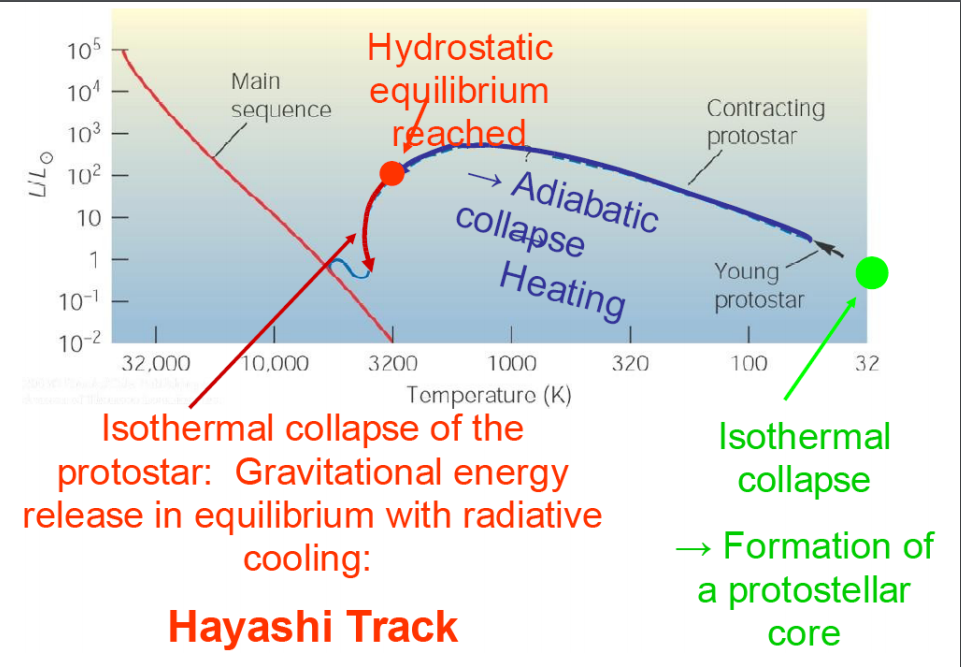
\includegraphics[width=13cm]{images/ewolucjaGwiazdHR.png}
                \end{center}
                Tak długo jak formując się gwiazda jest w całości konwektywna przebiega w dół po tzw. \textbf{ścieżce Hayasiego}. Kiedy włącza się transport promienisty, ścieżka zakręca na diagramie w lewo, aż w końcu osiąga ciąg główny. Czas trwania tego procesu zawiera się w przedziale od 10 tys. do 100 mln. lat. Dodatkowo \textbf{twierdzenie Vogta-Russella} mówi o tym, że gwiazda o ustalonej masie i składzie chemicznym trafia w ściśle określony punkt na ciągu głównym. W trakcie procesu formowania się gwiazdy wokół niej zwykle tworzy się \textbf{dysk protoplanetarny}, a wzdłuż osi rotacji wyrzucane są strumienie materii zwane \textbf{dżetami}.
            \subsubsection{Etap II: gwiazda świeci na koszt energii nuklearnej}
                W tej fazie gwiazda stabilizuje się na długi czas w porównaniu z procesem formowania się jej lub świecenia paliwem innym niż wodór. W jądrze stopniowo zmienia się skład chemiczny. W miarę spadku obfitości wodoru rośnie gęstość, ciśnienie i temperatura w centrum gwiazdy – jądro kurczy się reagując na zmianę składu chemicznego. W wyniku tych zmian gwiazd ,,wędruje'' po wykresie H-R (nadal pozostając w ciągu głównym) – stąd wynika szerokość pasu ciągu głównego na tym wykresie. Im bardziej gwiazda do góry i na prawo pasa ciągu głównego tym bliżej jej do wyczerpania paliwa wodorowego. Gdy zaczyna brakować paliwa wodorowego, gwiazda może zainicjować w swoim jadrze zainicjować syntezę cięższych jąder. Jednak spalanie takich jąder wiąże się z mniejszym zyskiem energetycznym. Żeby utrzymać równowagę termodynamiczną takie paliwo jest spalane szybciej – wyczerpuje się szybciej. Co więcej wymagany jest istotny wzrost temperatury – tylko pod tym warunkiem zachodzić może reakcja – wymogowi temu mogą sprostać wystarczająco masywne gwiazdy. Kolejnym problemem jest to, że w przypadku gwiazd zasilanych węglem lub cięższymi jądrami, sporą część energii reakcji unoszą neutrina powstające w wyniku spontanicznych przemian \(\beta\). Przy jeszcze cięższych jądrach kluczową role odgrywają cząstki \(\alpha\) będące produktami reakcji fotodezintegracji jąder (foton gamma rozbijający jądro). Poniżej infografika ilustrująca jak zmieniają sie parametry jąder gwiazd pod wpływem zmiany składu chemicznego:
                \begin{center}
                    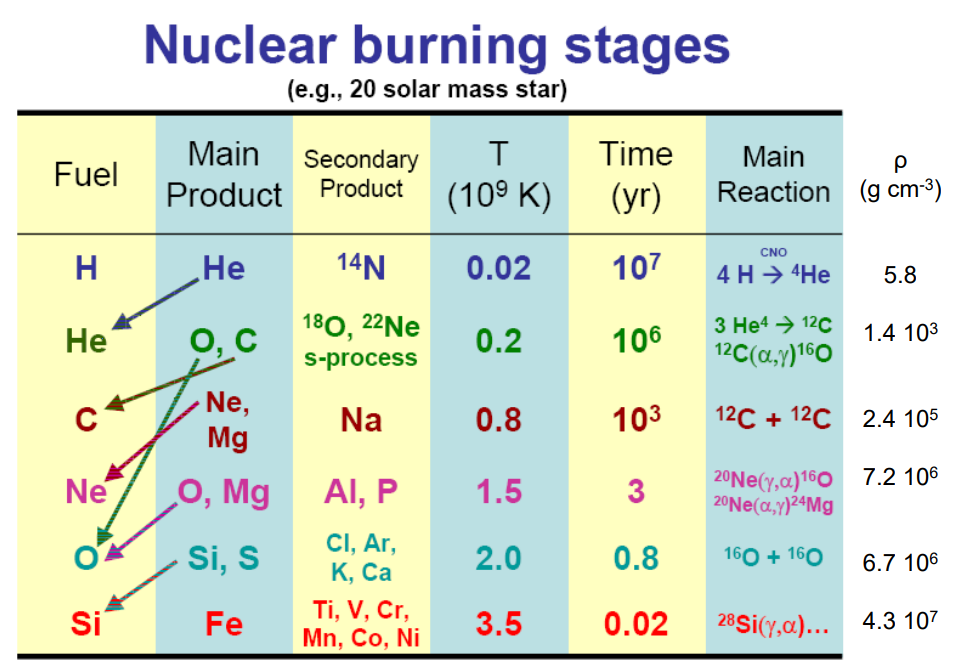
\includegraphics[width=13cm]{images/skladJadroGwiazda.png}
                \end{center}
        \subsection{Nukleosynteza}
            \textbf{Nukleosynteza} to proces powstawania pierwiastków. Jak widać na powyższej tabeli większość pierwiastków wytwarzana jest wewnątrz gwiazd. Jednak jak to się dzieje, że powstają także jądra pierwiastków cięższych o żelaza, mimo że jest to proces endoenergetyczny? Kluczową reakcją jest \textbf{wychwyt neutronu} – jądro wyłapuje neutron. Innym ważnym procesem jest \textbf{rozpad \(\beta\)} – zwiększa ilość protonów o jeden kosztem neutronu. Relacja pomiędzy tymi procesami określa możliwości nukleosyntetyczne gwiazdy. W szczególności wyróżnia się
            \begin{itemize}
                \item \textbf{proces s} –
            \end{itemize}
\end{document}